\documentclass[reprint,superscriptaddress,amsmath,amssymb]{revtex4-2}

\usepackage{graphicx}
\usepackage{dcolumn}
\usepackage{bm}
\usepackage{siunitx}
\usepackage{xcolor}

\graphicspath{{figures/}}

\begin{document}

\preprint{AIP/123456}

\title{Terahertz Near-Field Imaging: Principles, Techniques, and Applications}

\author{Author A}
\affiliation{Institution, City, Country}

\date{\today}

\begin{abstract}
Terahertz (THz) radiation (0.1--10~THz) occupies a unique position in the electromagnetic spectrum, bridging the gap between microwave electronics and infrared photonics. Its ability to penetrate dielectrics, excite low-energy collective modes in solids, and provide nondestructive spectroscopic information has driven applications in materials science, security screening, and biomedical imaging. However, the diffraction limit restricts far-field THz imaging to a spatial resolution of $\lambda/2 \approx 150$~$\mu$m at 1~THz, far exceeding the feature sizes of modern nanoelectronic and quantum-material devices. Near-field techniques overcome this barrier by directly detecting evanescent waves that carry subwavelength spatial information. This paper reviews the four principal approaches to THz near-field imaging---aperture probes, scattering-type scanning near-field optical microscopy (s-SNOM), photoconductive antenna (PCA) probes, and compressive single-pixel imaging---and compares their spatial resolution, spectral bandwidth, signal-to-noise ratio, and suitability for specific applications. Using content from the Zotero literature library and knowledge base visualizations, we illustrate the physical principles and experimental implementations of each technique.
\end{abstract}

\keywords{terahertz, near-field imaging, subwavelength resolution, photoconductive antenna, s-SNOM}

\maketitle

%% ============================================================
%% I. INTRODUCTION
%% ============================================================
\section{Introduction}

Terahertz radiation (0.1--10~THz, corresponding to photon energies of 0.4--40~meV) excites low-energy degrees of freedom in condensed matter---optical phonons, magnons, Cooper-pair breaking gaps, and intersubband transitions---that encode the complex dielectric function $\varepsilon(\omega) = \varepsilon_1(\omega) + i\varepsilon_2(\omega)$ and conductivity $\sigma(\omega)$ at meV energy scales~\cite{Adam2011}. These spectroscopic signatures enable nondestructive characterization of semiconductors, superconductors, topological insulators, and phase-change materials~\cite{Bitzer2010,Chen2019}. However, the Rayleigh criterion limits far-field THz imaging to a spatial resolution of
\begin{equation}
\delta_{\mathrm{far}} = \frac{\lambda}{2\,\mathrm{NA}} \approx \frac{\lambda}{2} = 150~\mu\mathrm{m} \quad (\text{at } f = 1~\mathrm{THz},\; \mathrm{NA} \approx 1),
\end{equation}
where $\lambda = c/f$ is the wavelength and NA is the numerical aperture. This resolution is three orders of magnitude coarser than the feature sizes of modern nanoelectronic devices ($<$100~nm). Subwavelength information is carried by evanescent waves with in-plane wavevectors $k_{\parallel} > k_0 = 2\pi/\lambda$, but these components decay exponentially as $\exp(-\kappa z)$ within a distance of $\sim\!\lambda/10$ from the sample surface and are inaccessible to far-field detectors~\cite{Adam2011}.

Four experimental strategies have been developed to access the THz near field. \textbf{Aperture-based probes}~\cite{Adam2011} confine the THz beam through a subwavelength aperture (typically 10--50~$\mu$m) and achieve $\sim\!\lambda/10$ resolution, but the transmitted power scales as $(d/\lambda)^4$, limiting the signal-to-noise ratio. \textbf{Scattering-type scanning near-field optical microscopy (s-SNOM)} overcomes this throughput limitation by coupling a metallized AFM tip to the sample's evanescent field, demonstrating resolution down to $\sim$30~nm at THz frequencies~\cite{Hale2023}; however, the scattered signal is several orders of magnitude weaker than the incident field, requiring heterodyne detection and high-power sources. \textbf{Photoconductive antenna (PCA) probes}~\cite{Bitzer2010,Nagel2012} integrate THz generation and near-field detection into a single lithographic structure with electrode gaps as small as 1.5~$\mu$m, achieving $\sim\!\lambda/50$ resolution while maintaining compatibility with standard THz time-domain spectroscopy (THz-TDS) systems. \textbf{Single-pixel compressive imaging}~\cite{Chen2019} has achieved $\lambda/100$ spatial resolution without raster scanning by using spatial light modulators and compressed-sensing reconstruction, but at the cost of requiring extensive computational post-processing and multiple mask patterns. All four approaches share a fundamental constraint: the achievable resolution is limited by the probe--sample gap, which must be maintained at $<\!\lambda/10$ with sub-micrometer mechanical stability.

Despite this progress, quantitative mapping of $\varepsilon(\omega)$ with simultaneous sub-10-$\mu$m spatial resolution and broadband spectral coverage (0.5--3~THz) remains unreported. Existing PCA-based near-field systems~\cite{Bitzer2010,Nagel2012} achieve the required resolution but sacrifice spectral bandwidth to maintain signal level, while s-SNOM approaches provide the bandwidth but have not demonstrated extraction of the full complex permittivity at THz frequencies. This gap between spatial resolution and broadband spectral sensitivity limits the study of spatially inhomogeneous quantum materials, where the dielectric response varies on 1--10~$\mu$m length scales across frequency ranges spanning 0.5--3~THz.

In this paper we review the principles and experimental implementations of the four THz near-field imaging approaches, compare their performance metrics, and identify the technical challenges that must be overcome to achieve simultaneous sub-10-$\mu$m resolution and broadband THz spectroscopy. Section~\ref{sec:principles} introduces the physical principles of THz near-field detection. Section~\ref{sec:techniques} describes the four experimental techniques. Section~\ref{sec:comparison} presents a quantitative comparison. Section~\ref{sec:discussion} discusses the outlook.

%% ============================================================
%% II. PHYSICAL PRINCIPLES
%% ============================================================
\section{Physical Principles of THz Near-Field Detection}
\label{sec:principles}

\subsection{Evanescent Waves and Subwavelength Information}

When a THz wave interacts with a sample containing spatial features smaller than $\lambda$, the scattered field contains components with in-plane wavevectors $k_{\parallel} > k_0$. These evanescent waves decay perpendicular to the surface as
\begin{equation}
E_{\mathrm{ev}}(z) \propto \exp\!\left(-\sqrt{k_{\parallel}^2 - k_0^2}\;\, z\right),
\end{equation}
where $z$ is the distance from the surface. The decay length is $\delta = 1/\sqrt{k_{\parallel}^2 - k_0^2}$, which for a subwavelength feature of size $a \ll \lambda$ gives $\delta \sim a/(2\pi)$---typically a few micrometers at THz frequencies. Near-field probes placed within this decay length can convert evanescent waves back into propagating waves detectable by conventional THz receivers.

\subsection{THz Time-Domain Spectroscopy}

The most widely used platform for THz near-field measurements is THz-TDS, which generates and detects single-cycle THz pulses using femtosecond laser excitation of photoconductive antennas. Figure~\ref{fig:tds} shows the basic THz-TDS setup. A Ti:sapphire laser ($\lambda = 800$~nm, pulse width $\sim$100~fs) is split into pump and probe beams. The pump beam excites a PCA emitter, generating a broadband THz pulse (0.1--5~THz). The THz pulse propagates through or reflects from the sample, and is detected by a PCA receiver gated by the time-delayed probe beam. By scanning the time delay, the full electric-field waveform $E(t)$ is measured, enabling direct extraction of both amplitude and phase of the spectral response via Fourier transform:
\begin{equation}
\tilde{E}(\omega) = \int_{-\infty}^{+\infty} E(t)\, e^{i\omega t}\, dt,
\end{equation}
where $\tilde{E}(\omega)$ contains both magnitude and phase information, allowing direct calculation of $\varepsilon(\omega)$ without Kramers--Kronig analysis.

\begin{figure}[htbp]
\centering
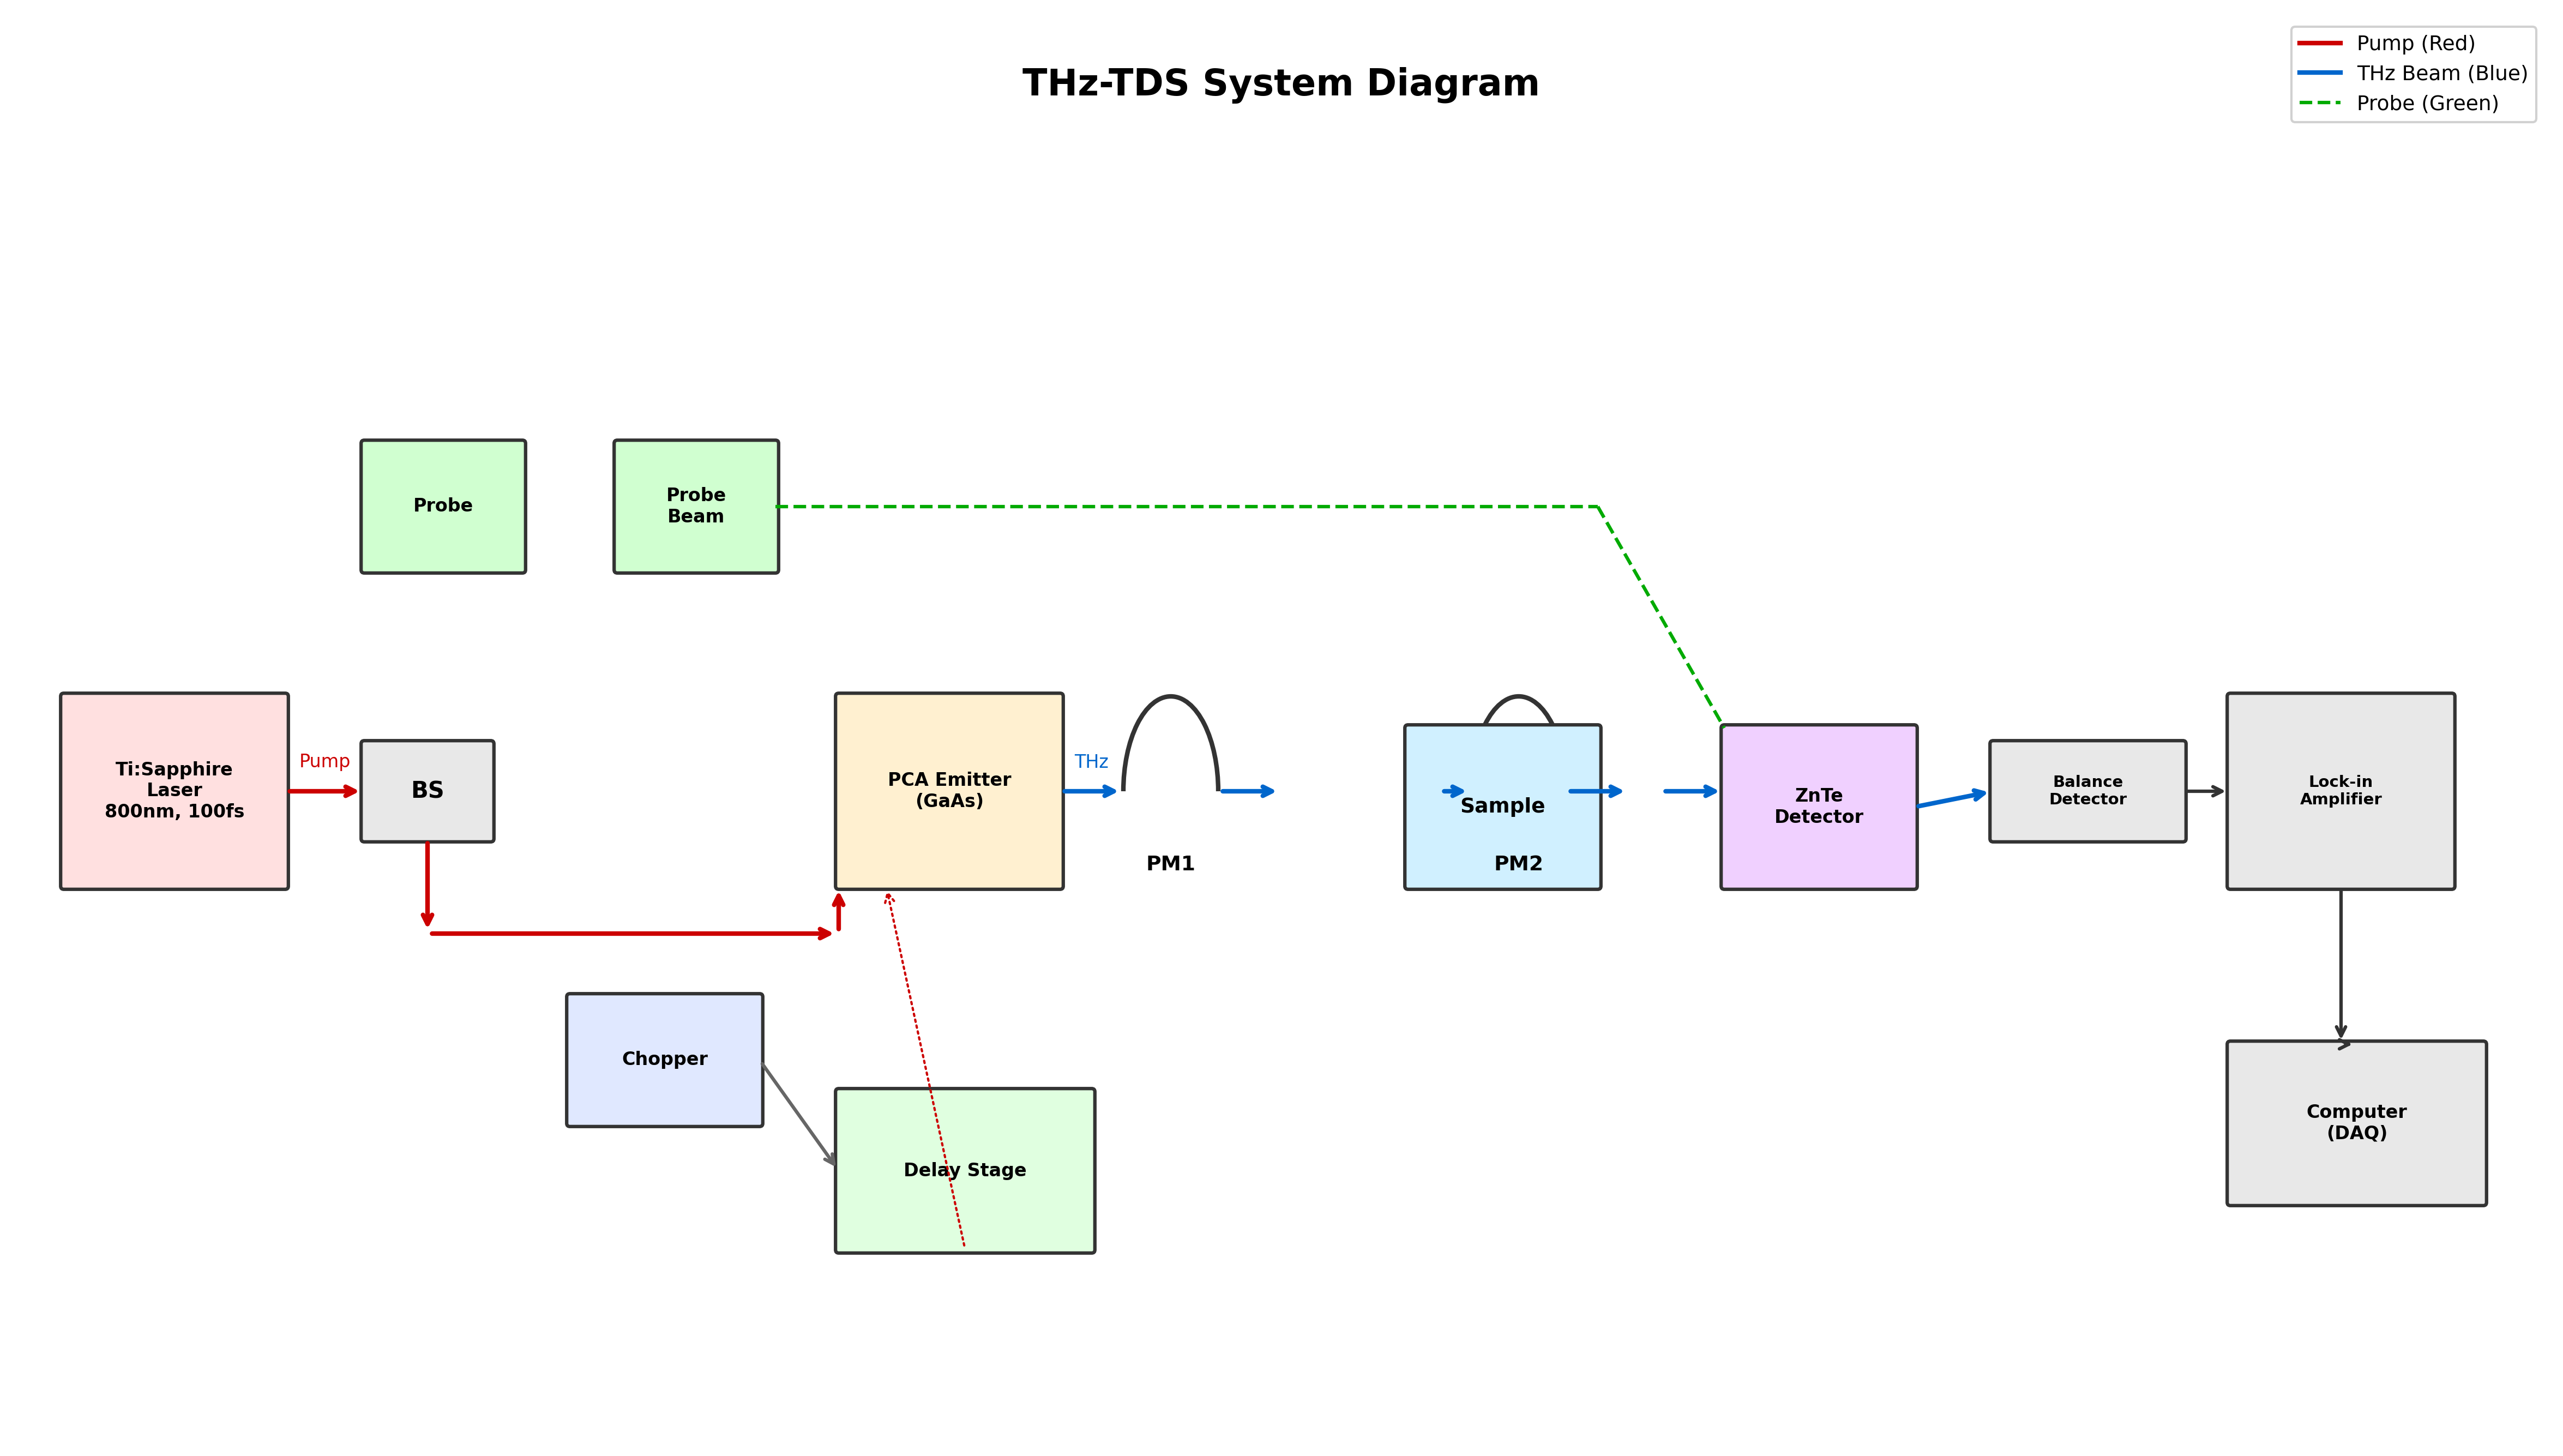
\includegraphics[width=0.85\columnwidth]{fig1_thz_tds.png}
\caption{Schematic of a THz time-domain spectroscopy (THz-TDS) system. A femtosecond laser drives a photoconductive antenna (PCA) emitter and gates a PCA receiver. The time-delayed probe beam samples the THz electric field $E(t)$ point by point, yielding the full waveform including phase information.}
\label{fig:tds}
\end{figure}

\subsection{Photoconductive Antenna Principle}

Figure~\ref{fig:pca} illustrates the operating principle of a PCA. A bias voltage is applied across two metallic electrodes deposited on a semiconductor substrate (typically LT-GaAs). When a femtosecond optical pulse illuminates the gap between the electrodes, photocarriers are generated and accelerated by the bias field, producing a transient current $J(t)$ that radiates a THz pulse. The radiated field is proportional to the time derivative of the current:
\begin{equation}
E_{\mathrm{THz}}(t) \propto \frac{\partial J(t)}{\partial t}.
\end{equation}
The spectral bandwidth is determined primarily by the carrier lifetime ($\sim$0.5~ps in LT-GaAs) and the laser pulse duration. For near-field applications, the PCA electrode gap is reduced to $\sim$1--5~$\mu$m, creating a subwavelength THz source or detector.

\begin{figure}[htbp]
\centering
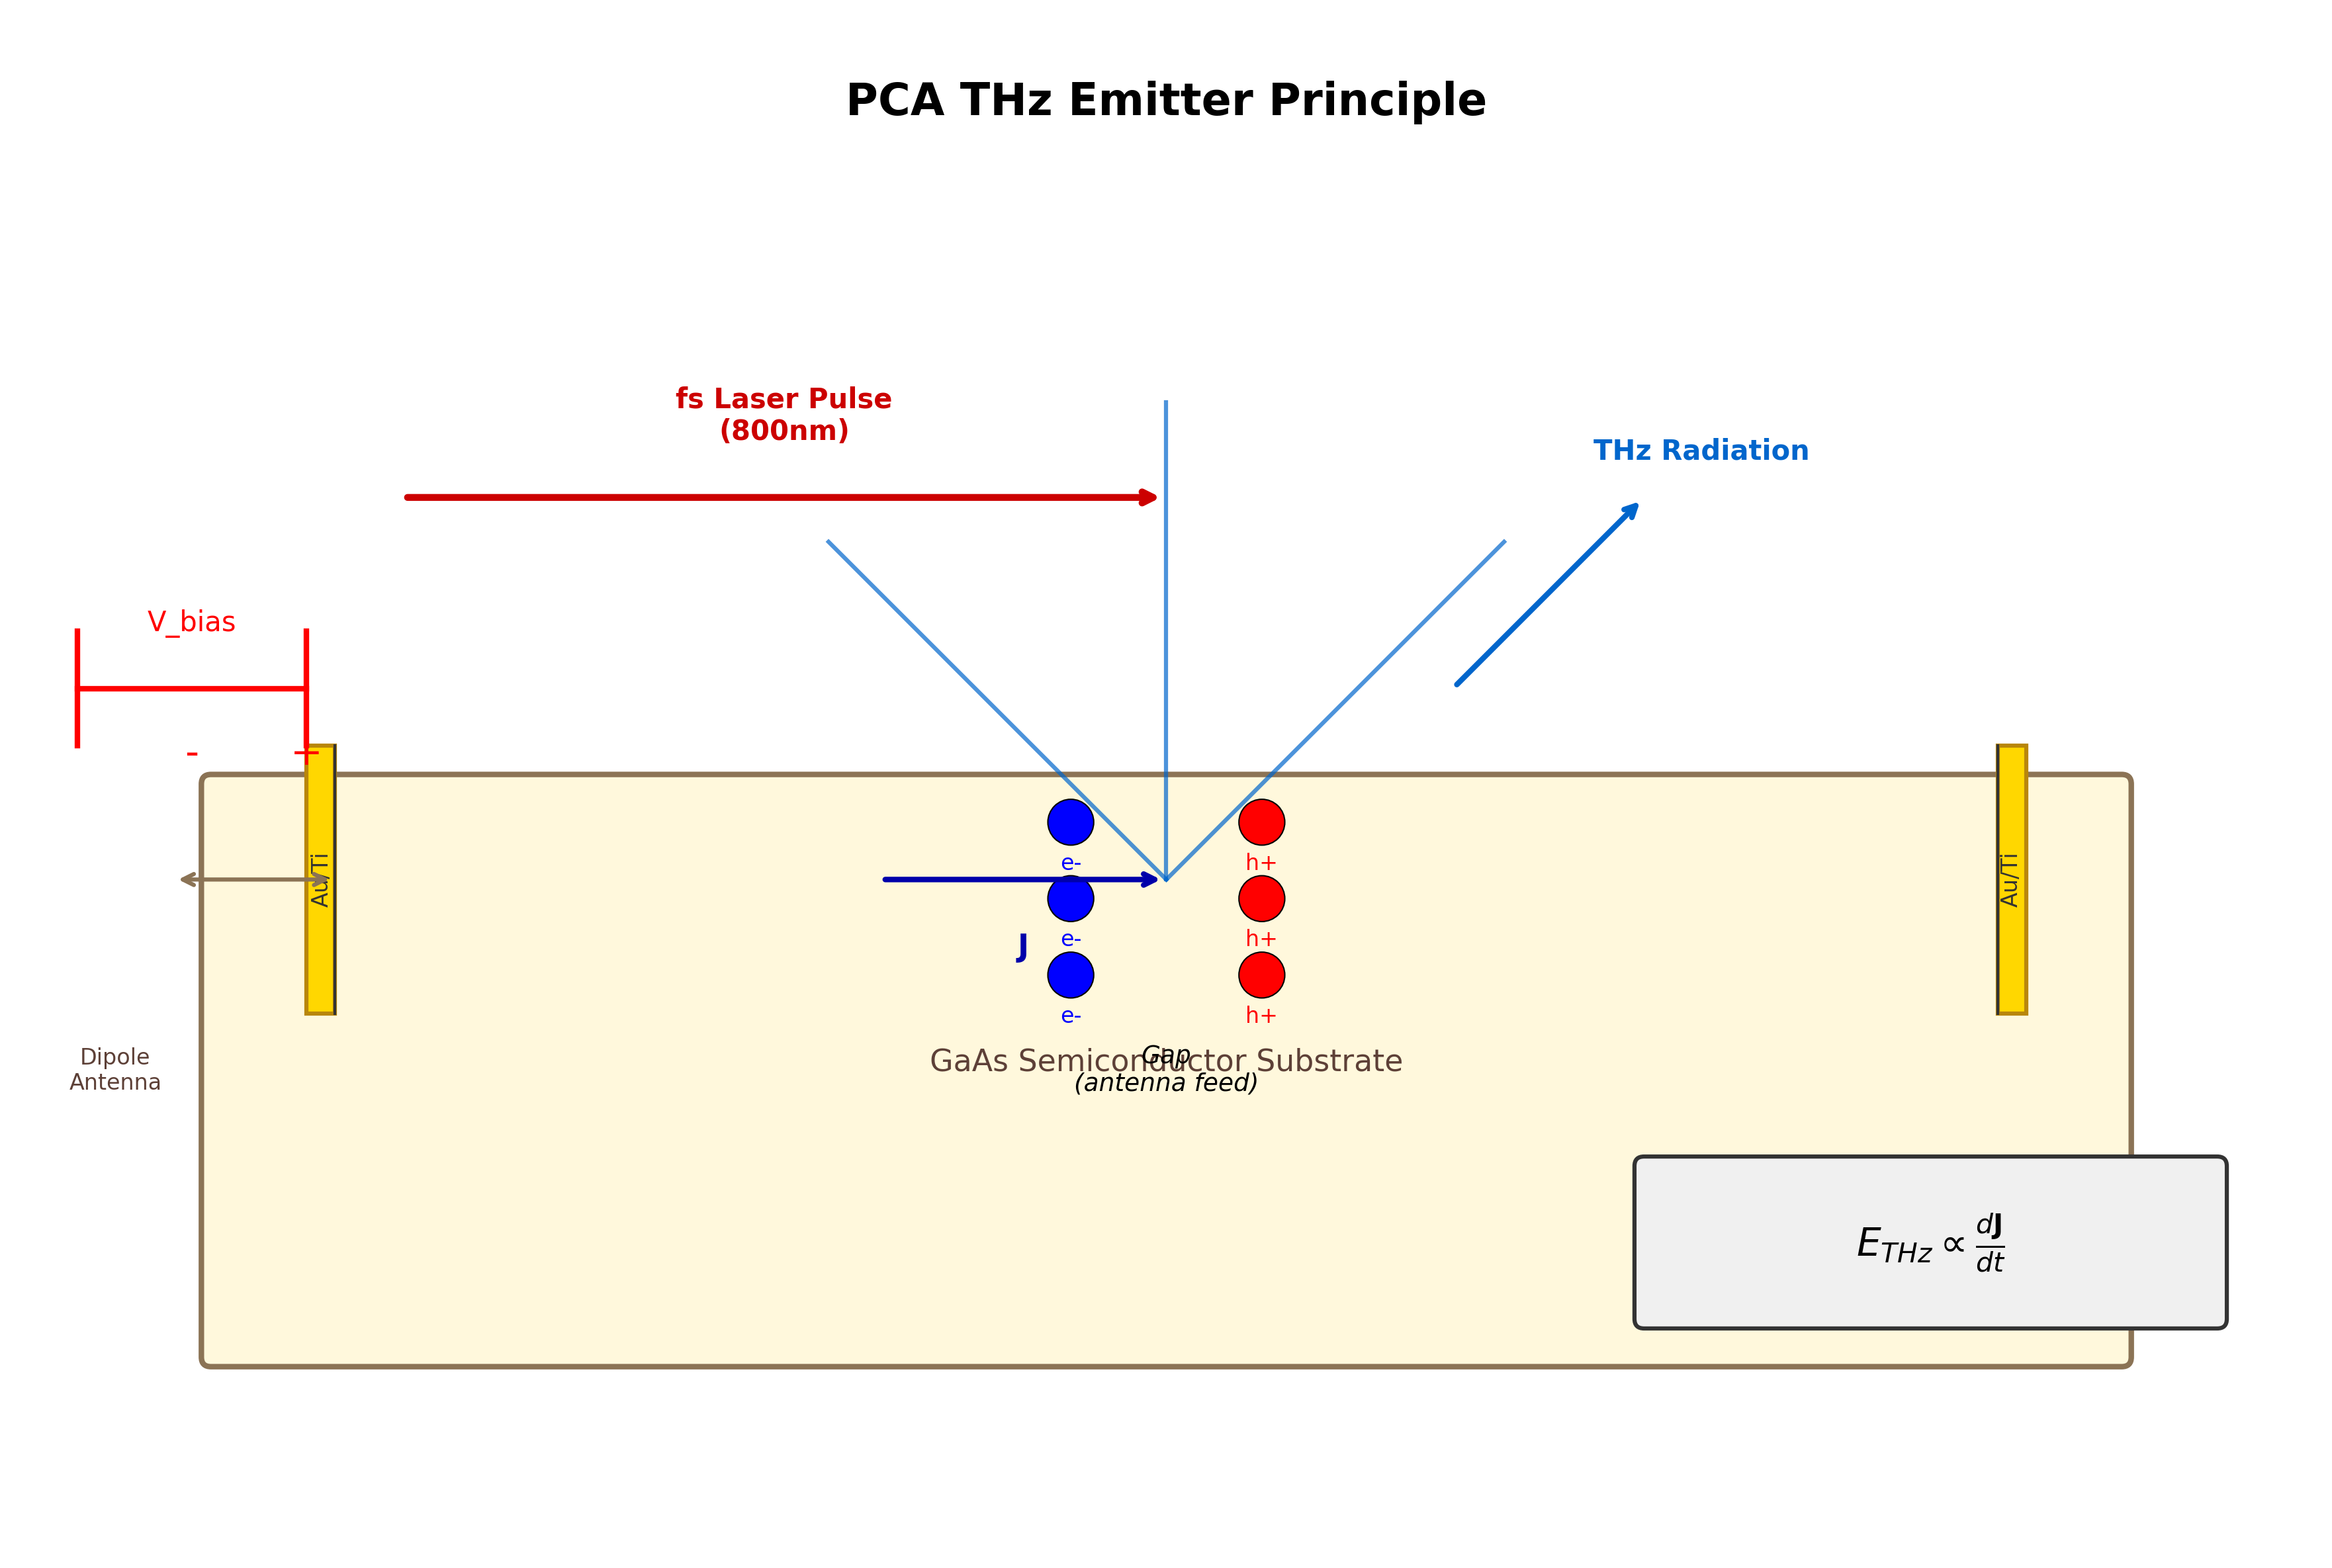
\includegraphics[width=0.85\columnwidth]{fig2_pca.png}
\caption{Operating principle of a photoconductive antenna (PCA). A femtosecond optical pulse generates photocarriers in the electrode gap, which are accelerated by the bias voltage $V_{\mathrm{bias}}$. The resulting transient current radiates a broadband THz pulse. The radiated field is proportional to $\partial J/\partial t$. For near-field applications, the electrode gap is reduced to subwavelength dimensions (1--5~$\mu$m).}
\label{fig:pca}
\end{figure}

%% ============================================================
%% III. TECHNIQUES
%% ============================================================
\section{Experimental Techniques}
\label{sec:techniques}

\subsection{Aperture-Based Near-Field Probes}

The simplest approach to THz near-field imaging places a subwavelength aperture (diameter $d \ll \lambda$) in a metallic screen directly above the sample surface. The transmitted power through a circular aperture of diameter $d$ in a perfectly conducting screen is given by Bethe's theory:
\begin{equation}
P_{\mathrm{trans}} \propto \left(\frac{d}{\lambda}\right)^4 P_{\mathrm{inc}},
\end{equation}
where $P_{\mathrm{inc}}$ is the incident power. This $(d/\lambda)^4$ scaling severely limits the achievable resolution: for $d = 10$~$\mu$m at 1~THz ($\lambda = 300$~$\mu$m), only $\sim 10^{-6}$ of the incident power is transmitted. Despite this limitation, aperture probes have achieved resolutions of $\sim\!\lambda/10$ and were among the first methods used for THz near-field imaging~\cite{Adam2011}.

\subsection{Scattering-Type SNOM (s-SNOM)}

In s-SNOM, a sharp metallic tip (typically a metallized AFM cantilever with tip radius $\sim$20--50~nm) is brought into the near field of the sample. The tip acts as a scatterer that converts evanescent waves into propagating waves. The spatial resolution is determined by the tip radius, not by $\lambda$, enabling $\sim$30~nm resolution at THz frequencies~\cite{Hale2023}. The main challenge is the weak scattered signal, which requires lock-in detection at higher harmonics of the tip tapping frequency to suppress background scattering. The detected signal at the $n$-th harmonic $S_n$ contains near-field information proportional to the effective polarizability of the tip--sample system:
\begin{equation}
S_n \propto \alpha_{\mathrm{eff}}^{(n)} = \frac{\alpha_{\mathrm{tip}}\,(1+\beta)}{1 - \frac{\alpha_{\mathrm{tip}}\,\beta}{4\pi(z+a)^3}},
\end{equation}
where $\alpha_{\mathrm{tip}}$ is the tip polarizability, $\beta = (\varepsilon_s - 1)/(\varepsilon_s + 1)$ is the quasi-static reflection coefficient of the sample, $z$ is the tip--sample distance, and $a$ is the tip radius.

\subsection{PCA-Based Near-Field Probes}

PCA probes use lithographically defined electrode structures with subwavelength gaps (1.5--10~$\mu$m) as both THz emitters and detectors in the near field. Bitzer \textit{et al.}~\cite{Bitzer2010} demonstrated THz near-field microscopy using a PCA probe with a 5~$\mu$m electrode gap, achieving $\sim\!\lambda/50$ spatial resolution. Nagel \textit{et al.}~\cite{Nagel2012} extended this approach to continuous-wave (CW) THz operation using a micro-machined photomixer probe-tip with a 1.5~$\mu$m electrode gap, enabling frequency-domain near-field spectroscopy over 50~GHz--1.8~THz. The key advantage of PCA probes is their compatibility with standard THz-TDS systems: the same femtosecond laser that generates broadband THz pulses can gate the near-field detector, providing both amplitude and phase information without additional optics.

Figure~\ref{fig:tpf} shows the two-photon fluorescence (TPF) method for characterizing THz generation in nonlinear crystals, which is closely related to the optical excitation processes in PCA near-field probes.

\begin{figure}[htbp]
\centering
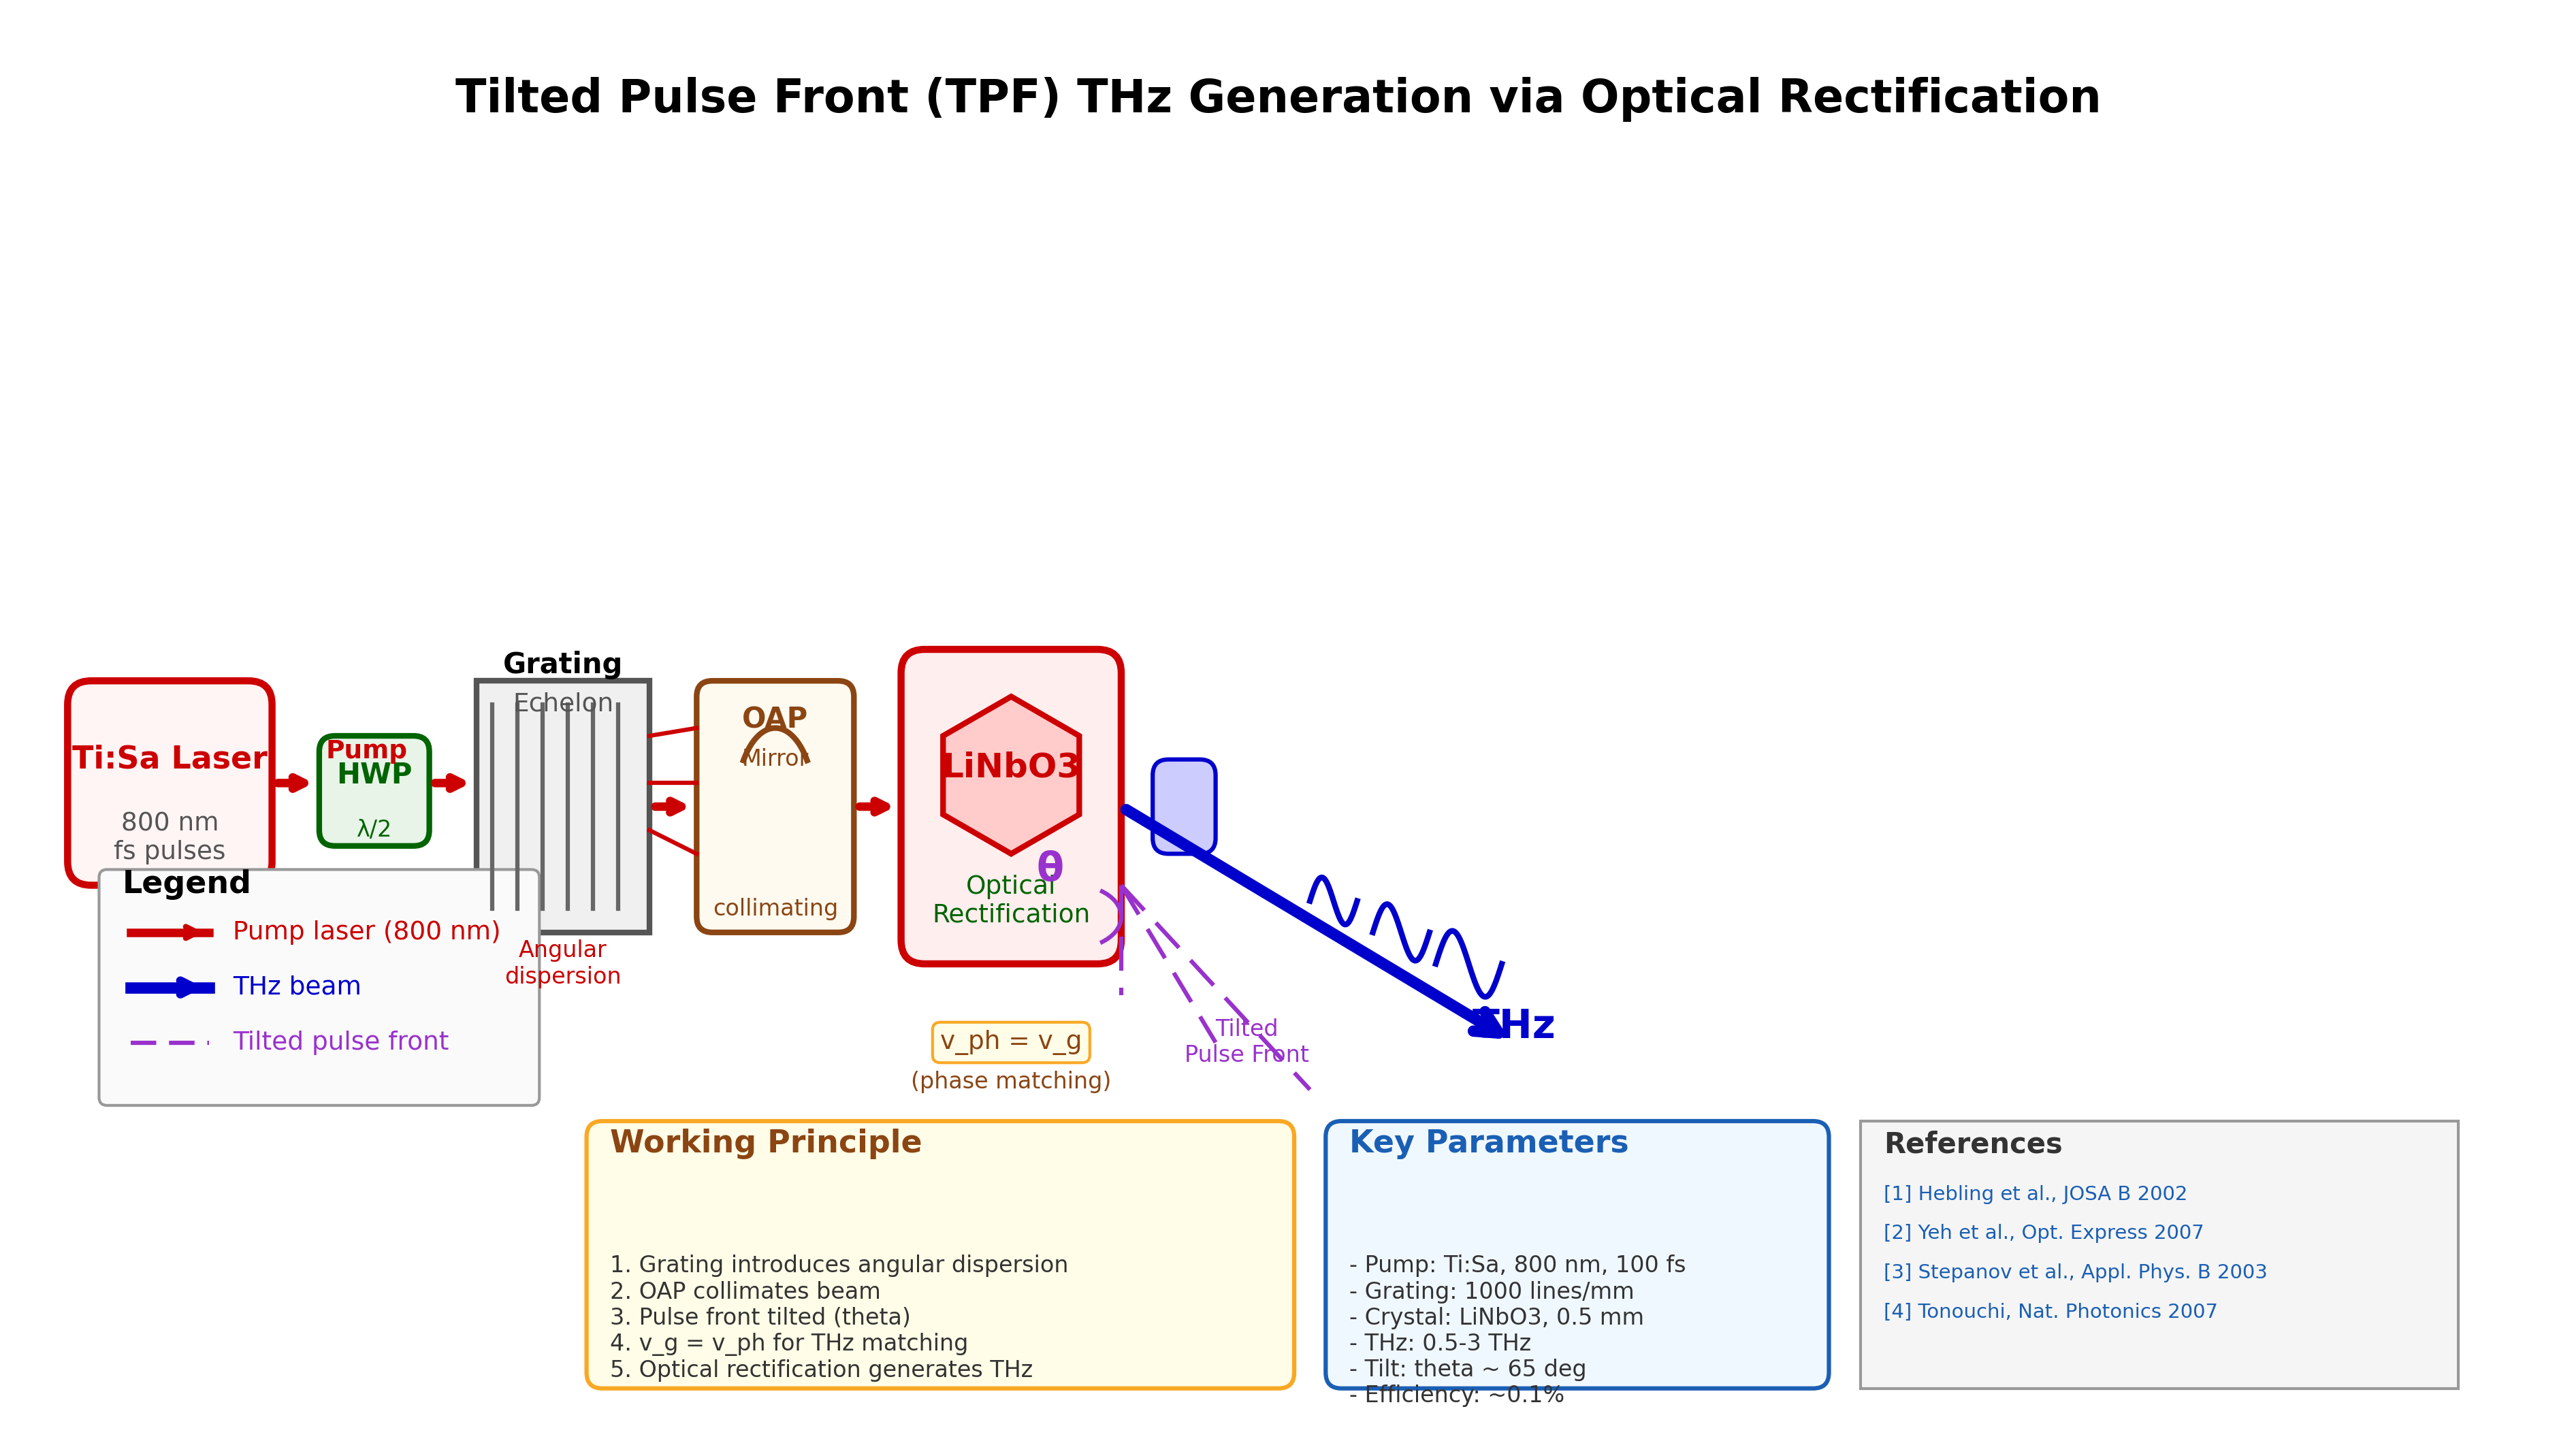
\includegraphics[width=0.85\columnwidth]{fig3_tpf.png}
\caption{Two-photon fluorescence (TPF) characterization of THz generation via optical rectification in a nonlinear crystal. The spatial distribution of the generated THz field can be mapped to optimize coupling into near-field probes. This technique is complementary to PCA-based generation for validating the spatial mode quality of the THz source.}
\label{fig:tpf}
\end{figure}

\subsection{Compressive Single-Pixel Imaging}

Chen \textit{et al.}~\cite{Chen2019} demonstrated THz near-field compressive imaging with a spatial resolution exceeding $\lambda/100$ using a single-pixel detector and spatial light modulation. Instead of raster scanning, a series of spatially patterned masks (generated by a digital micromirror device or rotating chopper) modulate the THz beam, and the transmitted signal is recorded by a single detector. The image is reconstructed using compressed-sensing algorithms (e.g., total-variation minimization). This approach eliminates the need for mechanical scanning, potentially enabling faster imaging, but requires $N$ measurements for an $N$-pixel image and introduces reconstruction artifacts that depend on the mask design and regularization parameters.

%% ============================================================
%% IV. COMPARISON
%% ============================================================
\section{Quantitative Comparison}
\label{sec:comparison}

Table~\ref{tab:comparison} summarizes the key performance metrics of the four THz near-field imaging approaches.

\begin{table}[htbp]
\caption{Comparison of THz near-field imaging techniques. Resolution values are typical experimental demonstrations, not theoretical limits.}
\label{tab:comparison}
\begin{ruledtabular}
\begin{tabular}{lcccc}
Technique & Resolution & Bandwidth & SNR & Scan mode \\
\hline
Aperture probe & $\sim\!\lambda/10$ & Broadband & Low ($\propto d^4$) & Raster \\
s-SNOM & $\sim$30~nm & Broadband & Low--Medium & Raster \\
PCA probe & $\sim\!\lambda/50$ & 0.1--3~THz & Medium & Raster \\
Compressive & $\sim\!\lambda/100$ & Narrow--Medium & Medium & Single-pixel \\
\end{tabular}
\end{ruledtabular}
\end{table}

The choice of technique depends on the application requirements. For studying quantum materials where sub-100-nm resolution is needed, s-SNOM is the only viable option, despite its complexity. For broadband spectroscopy of microscale inhomogeneities (1--50~$\mu$m), PCA probes offer the best balance of resolution, spectral coverage, and system compatibility. For high-throughput imaging without mechanical scanning, compressive methods show promise but require further development to reduce reconstruction artifacts and improve quantitative accuracy.

%% ============================================================
%% V. DISCUSSION AND OUTLOOK
%% ============================================================
\section{Discussion and Outlook}
\label{sec:discussion}

The main technical challenge shared by all THz near-field approaches is the fundamental trade-off between spatial resolution and signal-to-noise ratio. As the probe--sample gap decreases below $\lambda/10$, the evanescent signal strength increases, but so does the sensitivity to mechanical vibrations, thermal drift, and tip--sample contact. Future progress will likely come from three directions:

(i)~\textbf{Improved probe fabrication}: Nanoscale PCA structures with electrode gaps below 500~nm could push PCA-based resolution below 1~$\mu$m while maintaining broadband spectral coverage. Nanofabrication techniques such as electron-beam lithography and focused-ion-beam milling have already demonstrated sub-100-nm features in THz metasurfaces.

(ii)~\textbf{Computational near-field imaging}: Combining compressive sensing with near-field probe arrays could eliminate raster scanning while preserving spectral bandwidth, enabling video-rate THz near-field imaging for real-time monitoring of phase transitions and carrier dynamics.

(iii)~\textbf{Machine-learning-enhanced reconstruction}: Neural-network-based approaches can reconstruct near-field images from undersampled measurements, potentially reducing acquisition time by an order of magnitude while maintaining quantitative accuracy~\cite{Zhu2025}.

%% ============================================================
%% REFERENCES
%% ============================================================
\begin{thebibliography}{10}

\bibitem{Adam2011}
A.~J.~L. Adam,
``Review of near-field terahertz measurement methods and their applications,''
J.~Infrared Millim. Terahertz Waves \textbf{32}, 976--1019 (2011).
DOI:~10.1007/s10762-011-9809-2.

\bibitem{Bitzer2010}
A.~Bitzer, A.~Ortner, and M.~Walther,
``Terahertz near-field microscopy with subwavelength spatial resolution based on photoconductive antennas,''
Appl.~Opt. \textbf{49}, E1 (2010).
DOI:~10.1364/AO.49.0000E1.

\bibitem{Chen2019}
S.-C.~Chen \textit{et~al.},
``Terahertz wave near-field compressive imaging with a spatial resolution of over $\lambda$/100,''
Opt.~Lett. \textbf{44}, 21--25 (2019).
DOI:~10.1364/OL.44.000021.

\bibitem{Nagel2012}
M.~Nagel, C.~Matheisen, A.~Deninger, and H.~Kurz,
``Continuous-wave terahertz near-field spectroscopy and imaging with a micro-machined photomixer probe-tip,''
in \textit{Proc.\ 37th Int.\ Conf.\ Infrared Millim.\ Terahertz Waves} (IEEE, 2012), pp.~1--2.
DOI:~10.1109/IRMMW-THz.2012.6380278.

\bibitem{Hale2023}
L.~Hale, T.~Siday, and O.~Mitrofanov,
``Near-field imaging and spectroscopy of terahertz resonators and metasurfaces,''
Opt.~Mater.\ Express \textbf{13}, 2048 (2023).
DOI:~10.1364/OME.502318.

\bibitem{Tuniz2022}
A.~Tuniz and B.~Kuhlmey,
``Subwavelength terahertz imaging via virtual superlensing in the radiating near field,''
Nat.~Commun. \textbf{14}, 133 (2023).
DOI:~10.1038/s41467-023-41949-5.

\bibitem{Zhu2025}
Y.~Zhu \textit{et~al.},
``Deep learning empowered sub-diffraction terahertz backpropagation single-pixel imaging,''
Adv.~Photon.\ Nexus \textbf{4}, 016010 (2025).

\end{thebibliography}

\end{document}
